\section{Одномерное уравнение диффузии}

В декартовых координатах:
\begin{equation} \label{diffusion_cartesian}
\dfrac{\partial u}{\partial t} - \nu \dfrac{\partial^2 u}{\partial x^2} = 0
\end{equation}

В цилиндрических координатах:
\begin{equation} \label{diffusion_cilinder}
    \dfrac{\partial \left( ru \right)}{\partial t} - \dfrac{\partial}{\partial r} \left(  \right)
\end{equation}


\subsection{Описание математической модели}
Параболическое

\subsection{Описание начальных и граничных условий}
Течение Куэтта

"Ступенька"
\subsection{Описание метода конечных разностей}


\subsection{Задача: Разгон жидкости в цилиндрической трубе}

\begin{figure}[H]
    \centering
    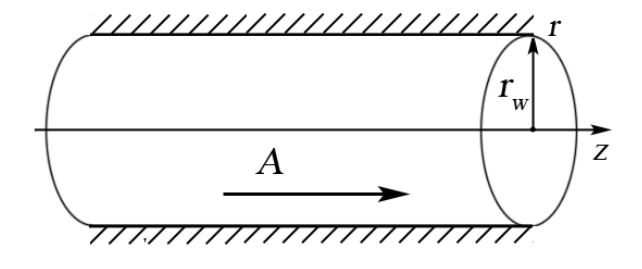
\includegraphics[width=0.5\linewidth]{fig/Рисунок_к_задаче.png}
    \caption{}
    \label{fig:task_fig}
\end{figure}

Течение описывается уравнением
\begin{equation} \label{tast_eq}
    \dfrac{\partial \left( ru \right)}{\partial t} - \dfrac{\partial}{\partial r} \left( r \nu \dfrac{\partial u}{\partial r} \right) - \dfrac{r}{\rho} \dfrac{\partial p}{\partial z} = 0
\end{equation}

Переход от консервативной (дивергентной) формы уравнения к обычной не является тождественным преобразованием, потому что 

Оператор Лапласа 

\begin{equation} \label{taskEquation}
\frac{\partial (ru)}{\partial t} - \frac{\partial}{\partial r} \left( r \nu \frac{\partial u}{\partial r} \right) - \frac{r}{\rho} \frac{\partial p}{\partial z} = 0
\end{equation}

\subsubsection*{Явная центральная схема}

\begin{equation} \label{taskFTCSderivation}
\begin{aligned}
r_i \frac{u_i^{n+1} - u_i^n}{\Delta t} - 
\nu \left(
r_{i+0.5} \frac{u_{i+1}^n - u_i^n}{\Delta r^2} -
r_{i-0.5} \frac{u_i^n - u_{i-1}^n}{\Delta^2}
\right) = Ar_i \\
\frac{r_i}{\Delta t} u_i^{n+1} = \frac{r_i}{\Delta t} u_i^n + 
\nu \frac{r_{i+0.5}}{\Delta r^2} u_{i+1}^n -
\nu \frac{r_{i+0.5}}{\Delta r^2} u_i^n - 
\nu \frac{r_{i-0.5}}{\Delta r^2} u_i^n +
\nu \frac{r_{i-0.5}}{\Delta r^2} u_{i-1}^n + Ar_i
\end{aligned}
\end{equation}

Введя следующее обозначение:
\begin{equation} \label{taskFTCS_briefly}
s = \nu \frac{\Delta t}{\Delta r^2 r_i},
\end{equation}
можем записать удобную для программной реализации формулу:
\begin{equation} \label{taskFTCS}
u_i^{n+1} = s\cdot r_{i-0.5}\cdot u_{i-1}^n -
s\left(r_{i-0.5} + r_{i+0.5} - \frac{1}{s}\right) u_i^n +
s \cdot r_{i+0.5} \cdot u_{i+1}^n + A\cdot \Delta t
\end{equation}

\subsubsection*{Двухшаговая схема Алена-Чена}


Предиктор:
\begin{equation} \label{taskPredictor}
\begin{aligned}
r_i \frac{\Tilde{u}_i^{n+1} - u_i^n}{\Delta t} - 
\nu \left(r_{i+0.5} 
\frac{u_{i+1}^{n} - \Tilde{u}_i^{n+1}}{\Delta r^2} - r_{i-0.5} \frac{\Tilde{u}_i^{n+1} - 
u_{i-1}^{n}}{\Delta r^2} 
\right) = Ar_i \\
\left( 
\nu \frac{r_{i-0.5}}{\Delta r^2} +
\frac{r_i}{\Delta t} +
\nu \frac{r_{i+0.5}}{\Delta r^2}
 \right)
\Tilde{u}_i^{n+1} =
\nu \frac{r_{i-0.5}}{\Delta r^2} u_{i-1}^n +
\frac{r_i}{\Delta t} u_i^n + 
\nu \frac{r_{i+0.5}}{\Delta r^2} u_{i+1}^n + Ar_i
\end{aligned}
\end{equation}

Введя следующие обозначения
\begin{equation} \label{taskDefinitions}
s_1 = 
\nu \frac{r_{i-0.5}}{\Delta r^2}, \;
s_2 = 
\frac{r_i}{\Delta t}, \;
s_3 =
\nu \frac{r_{i+0.5}}{\Delta r^2}, \;
s_4 = (s_1 + s_2 + s_3)^{-1},
\end{equation}
можем записать предиктор в компактной форме:
\begin{equation}
\label{taskShortPredictor}
\Tilde{u}_i^{n+1} = 
(s_1 u_{i-1}^n +
 s_2 u_i^n + 
 s_3 u_{i+1}^n + Ar_i) \cdot s_4
\end{equation}

Аналогичные выкладки для корректора:
\begin{equation} \label{taskPredictor}
\begin{aligned}
r_i \frac{u_i^{n+1} - u_i^n}{\Delta t} - \nu 
\left(r_{i+0.5} \frac{\Tilde{u}_{i+1}^{n+1} - u_i^{n+1}}{\Delta r^2} - r_{i-0.5} \frac{u_i^{n+1} - 
\Tilde{u}_{i-1}^{n+1}}{\Delta r^2} 
\right) = Ar_i \\
\left( 
\nu \frac{r_{i-0.5}}{\Delta r^2} +
\frac{r_i}{\Delta t} +
\nu \frac{r_{i+0.5}}{\Delta r^2}
 \right)
u_i^{n+1} =
\nu \frac{r_{i-0.5}}{\Delta r^2} \Tilde{u}_{i-1}^{n+1} +
\frac{r_i}{\Delta t} u_i^n + 
\nu \frac{r_{i+0.5}}{\Delta r^2} \Tilde{u}_{i+1}^{n+1} + Ar_i
\end{aligned}
\end{equation}



\begin{equation}
\label{taskShortCorrector}
u_i^{n+1} = 
(s_1 \Tilde{u}_{i-1}^{n+1} +
 s_2 u_i^n + 
 s_3 \Tilde{u}_{i+1}^{n+1} + Ar_i) \cdot s_4
\end{equation} 


